\documentclass[twocolumn]{atlantis-press}
\usepackage[dvips]{graphicx}
\usepackage[latin1]{inputenc}
\usepackage{amssymb,amsmath,array}
\usepackage{atlantis-press}
\usepackage{lmodern} % Times fonts

\graphicspath{ {imagens/} }

%***********************************************************************
% !!!! IMPORTANT NOTICE ON TEXT MARGINS !!!!!
%***********************************************************************
%
% Please avoid using DVI2PDF or PS2PDF converters: some undesired
% shifting/scaling may occur when using these programs
% It is strongly recommended to use the DVIPS converters, and to submit
% PS file. You may submit a PDF file if and only if you use ADOBE ACROBAT
% to convert your PS file to PDF.



%***********************************************************************
% !!!! USE OF THE Atlantis Press LaTeX STYLE FILE !!!!!
%***********************************************************************
%
% Some commands are inserted in the following .tex example file.  Therefore to
% set up your Atlantis Press submission, please use this file and modify it to insert
% your text, rather than staring from a blank .tex file.  In this way, you will
% have the commands inserted in the right place.


\begin{document}

\title{Location-Based Service to reduce the waiting time for taxi services}

\begin{aug}
\author[1]{Felipe A. L. Reis}
\author[2]{Marconi A. Pereira}
\author[1]{Paulo E. M. Almeida}
\affilation[1]{CEFET-MG - Centro Federal de Educa��o Tecnol�gica de Minas Gerais, Belo Horizonte, MG, Brazil}
\affilation[2]{UFSJ - Universidade Federal de S�o Jo�o Del-Rei, Ouro Branco, MG, Brazil}
\end{aug}

%
%
\maketitle

%
%
\begin{abstract}
One solution to increase the operational efficiency 
of the taxis systems is using location-based 
services (LBS) in order to choose the best cab 
available to service a request.
In this work are evaluated different algorithms 
for define the best cab, when the position of the 
vehicle and the passenger are known.
In tests, in a stationary system, it was observated, 
through simulation, a waiting time reduction and a 
decrease of the distance to response, when was used 
LBS algorithms instead of broadcasting methods - 
currently used to choose the taxi for service.

\emph{\textbf{\textit{(92 words (max 100))}}}
\end{abstract}

%
%
\begin{keywords}
Location-based services (LBS), urban taxi transportation,
real-time routing, assignment problems
\end{keywords}

%
%
\section{Introduction}
%
Taxi is a option of transportation, in urban areas, that offer 
quickness and comfort to the public. The taxi transportation 
systems suffers influence of different factors, that change its 
availability. Among then, its possible to mention:
%
\begin{itemize}
	\item Events such as concerts, parties and conferences generate
	strong demand at a specific point, usually
	concentrated in a small time interval (closing time);
	\item Rainy Days motivate people who usually move by walk, 
	subway or bus to use a cab, which generates a great sprayed 
	demand, that is, there isn't a concentration of users in a
	specific point;
	\item Rush times, where there is a peak traffic;
	\item Beginning or end of hollidays, when users choose to 
	travel the airports, bus or train stations.
\end{itemize}
%
The operation of taxi services, generally, is unsatisfactory 
as to its operational efficency. The reasons are related to the 
lack of methodology to serve request and th way how taxis 
systems is organized: phone call schedules, random search methods 
to take customers (taxi drivers and passenger look for each other) 
and use of taxi ranks. 
\cite{CHENG_QU}.

In search of effective improve of taxi services, it's necessary 
a balance between availability, number of requests by region and 
the knowledge of detailed information about preferences, traffic 
flow and access routes. The union of this informations can produce 
models that describes the behavior of taxi services. However, due 
their own characteristics - such as the number of cabs, authonomous 
stocatic demand in different locations and the absense of patterned 
behavior of drivers - creating those models of operation is 
feasible, even for representations average size \cite{CHENG_QU}.

A alternative solution for this scenario is using of trackers 
in the vehicles, that send location information of drivers and 
passengers. The location-based services can increase the 
operational efficiency: the knowledge of geographical location 
of cabs and passenger enables the choose of the best vehicle for 
each request, improving the global result of the system.

The use of global location technology with taxis request was 
already studied by \cite{LIAO} e \cite{XU_ET_AL}. In their papers, 
the request of taxis services is through telephone exchanges, 
where the client informs his own location and the operator 
identifies the closest cab to server the request. However, 
these papers do not describe the algorithms used for choosing 
the best taxi driver, or the winnings of each.

This paper seeks to evaluate the gain, at the overall average time, 
of the GPS-based algorithms compared to the broadcasting method - 
mainly used today, in order of vehicles. This work, seeks also 
to analyze how the distance affects the time of taxi waiting when 
to cab has already choose and how the increase/decrease of supply 
services changes the average time of the system. At least, this 
paper measures the processing time of the proposed algorithms.

%
%
\section{Background}
%
The taxis systems are everywhere: big cities, medium-sized cities 
and even small cities around the world has a infrastructure of 
these services. The taxi system meet demand of the native population 
and the tourist, that visit or works on this cities.

At the most of cities around the world, its possible to know that 
taxi services waste a large portion of time - about 50\% - waiting 
for passengers \cite{CHENG_QU}. Because of the righ rate of waste of 
time in taxis systems, there are a large number of studies that goal 
to improve the efficency of the services, without increased costs 
\cite{CHENG_QU}.

The use of geographical location with the data obtained by tracker, 
recently has been incorporated into dispatch systems \cit�{XU_ET_AL}. 
From the knowledge of the absolute position of a passenger, it's 
possible to know, accurately, data about products and options of 
services that interest possbile consumers \cite{RAO_MANAKAKIS}.

There are different techniques to find customers, since
random search methods to GPS-based methods, which is known 
the location of taxi drivers and passengers. 
The knowledge of the passengers and the cabs positions allow a 
big advantage of others methods: it's possible to choose the best 
vehicle fleet to meet every request more efficiently.
According \cite{XU_ET_AL}, the GPS-based method for order 
vehicles will be used more efficiently to meet the demands of 
taxi, when knowing the location of taxi drivers and passengers.

In general, location systems monitor the position of taxis by 
vehicle tracking. \cite{LIAO} and \cite{XU_ET_AL} describes 
real systems that store the absolute position of taxis cabs and, 
after a call to a dispatch center, define the best vehicle for 
the request, according to the client position.

Because of the growing use of smarthphones in the world, 
\textbf{\textit{verifcar fonte!!}}, plus de possible maintenance 
of this trend for the next years \textbf{\textit{verifcar fonte!!}},
it's possible to build systems that use the intergrated GSP / A-GPS 
trackers to locate vehicles and passengers. By the requests comming 
for this devices, the knowledge of taxi drivers and clients become 
innate e it's possible to provide taxi services with better 
efficency. 

%
%
\section{Algorithms}
%
\subsection{GPS-based algorithm with lower estimated time for service}
%
One of the options to choose the best taxi driver to server 
a request is the development of an algorithm that choose 
always the best vehicle whose time estimation
attendance is the lowest possible.

To choose the best cab, we have to estimate each travel time 
of each taxi cab, based on the real route between the cab 
and the passenger. There are, however, a problem in this 
simplified solution: the cost to evaluate all taxi cabs make 
the request processing so slow, due the complexity of 
routing algorithms. 

In order to decrease the response time, the pre-processing of 
taxi driver by linear euclidian distance to the client can 
decrease the processing time without affecting the quality 
of the algorithm. In this aproach, it's thought that exists 
a linerarity between the distance and time to attendance.

Using the euclidian distance, it's possible to classify by cabs 
by it's distance to the client. The first step is select taxis in 
a range of distance and order then by ascending distance. If there 
are no taxi drivers in a range defined at begin, the algorithm 
proceed as follows:

%
\begin{enumerate}
	\item Increase the range of distance to find taxis;
	\begin{enumerate}
		\item If at least one taxi was found in the new range, 
		the algorithm process the cabs found;
		\item Otherwise, the range is increase again;
		\begin{enumerate}
			\item If at least one taxi was found in the new range, 
		the algorithm process the cabs found;
			\item Otherwise, the algorithm concludes that there are 
			no cabbies near and puts the customer in queue;
		\end{enumerate}
	\end{enumerate}
\end{enumerate}
%
We can more easily understand the algorithm with the Figure
\ref{fig:circulos}. The taxi drivers are searched first in the 
green region of concentric circles 
\textbf{\textit{(substituir por hachurada 1)}}. If not found, 
they are search in the yellow region 
\textbf{\textit{(substituir por hachurada 2)}} and, finally,
if necessary, in the red region 
\textbf{\textit{(substituir por hachurada 3)}}. 
If no taxi is found, the algorithm puts the customer in queue.
%
\begin{figure}[!h]
	\centering
	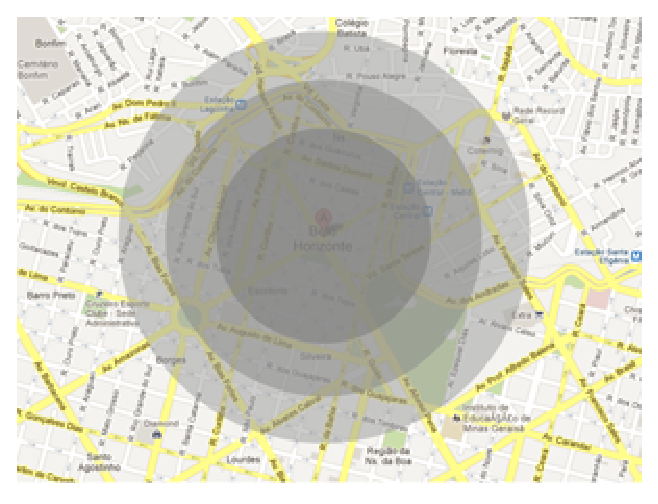
\includegraphics[scale=0.6]{circulos.eps}
	\caption{Method to filter taxis, by their distance to the customer.}
	\label{fig:circulos}
\end{figure}
%
Using the circles concept defined above, it's possible to 
limit the maximal distance that a cab will be evaluated to 
server a request. The maximal distance limit aim to prevent 
that taxi drivers too far from the customers can be choosen 
by the algoritm to serve a request. Far drivers will have to 
travel great distances and, it's possible that the profit don't 
pay the costs of drive to the passenger. Futhermore, the 
clients will wait for long time, that is not a good thing.

If the system using data filters, nevertheless, find a great 
number of taxi cabs fit for service, the system limit the near 
N drivers, further reducing processing. Among these drivers, 
the system will estimate each travel time to the client and 
define the reponsible for request.

In this article, in order to encapsulate the estimation process
time request was used to Google Maps API for obtaining
the lowest actual route. The filter of taxi driver is done by 
the a self algorithm.

%
\subsection{GPS-based algorithm with Euclidean distance}
%
An alternative algorithm to that described in the previous 
section is just use the Euclidean distance as a criterion for
choosing the best taxi driver.

Analysing this method, however, in a real situation, the 
euclidean distance can may prove ineficiency, since the nearest 
taxi, according this criterion, may take a longer travel to 
the client a little more distance, but uses a different route. 
It's possible to see this situation with the Figure 
\ref{fig:rota_taxista_cliente}. 
%
\begin{figure}[!h]
	\centering
	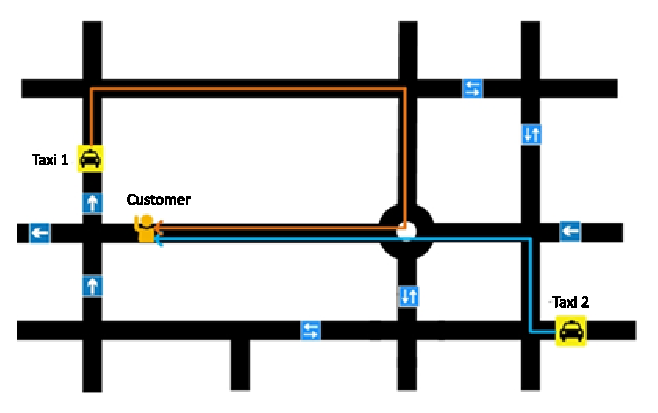
\includegraphics[scale=0.6]{rota_taxista_cliente.eps}
	\caption{Example of routes between taxis and a customer.}
	\label{fig:rota_taxista_cliente}
\end{figure}
%
In the last figure, it's possible to see clearly that Taxi 1 
is closer to Client 1 than Taxi 2, using euclidean distance 
algorithm. Nevertheless, Taxi 2 will travel a lower distance 
than Taxi 1 to serve the client.

Despite of the problems discussed above when using only the 
euclidean distance to define the best taxi, this solution has 
a considerably lower computational cost, and can deliver good 
results in the average case.

Simirarly to the first method with the lowest estimated time 
of service, it's defined a maximal distance range of taxis that 
can serve the request.

%
\subsection{Broadcasting method}
%
The broadcasting method is currently used for choice of 
the taxi driver responsible for meeting a client after a 
call to the call center. In that, the operator communicates, 
by radio, to the taxi drivers the location of the passenger. 
One of the taxi drivers near the customer confirms that is 
available and can serve the resquest. Then it's applied for 
the request.

The broadcasting method does not guarantee that the near driver 
will be choose nor the system is optimized to meet the demands: 
the driver who first answers the demand is the one that will 
serve the request. It's possible to conclude that the choice of 
the driver is carried out in a way of random, since the driver 
thats first response to the operator is choosen. 

To simulate this method, an algorithm was developed. In it, after 
a request, the algorithm selects a set of a near taxi drivers 
(using the limit of distance like the GPS-based algorithms) a draws 
a taxi cab. Through the draw, can represent the selection of the 
applied cabbie.

%
%
\section{Tests and Results}
%

The simulation engine designed to test the algorithms 
described is classified as Discrete Event Simulation.

Tests were performed for all algorithms under same conditions. 
Each method defined the best taxi driver to service, according 
to your own criteria. The time displacement of each taxi was c
omputed in each of the algorithms.

To calculate the average time service was used Google Maps API 
in order to estimate the travel time between taxi driver and the 
customers, since the use of real data is currently considered 
infeasible. This estimate was defined as time to serve a request. 
The simulator does not evaluate, at the tests, traffic informations.

%
\subsection{Taxi distribution}
%
To define the distribution of service demands in the area used 
as a representation of a city, we built a placement generator for 
taxis and passengers.

In it, it's evaluated the probability of a event in a peripherical 
area of the city is less than the probability of a event in the 
central region. This distribution represents a situation where 
a small place or a single place receives greater amounts of request. 
In large cities, at the most of times, several places concetrates 
the major number of requests, unlike a only single area. However, 
these usual behavior is complex to be modeled, especially when 
related to stochatic demand for taxi services \cite{CHENG_QU}.

The taxis cabs, likewise the demands were not distributed uniform. 
Using the same algorithm, they occupy, at most, the central region. 
The peripherical area has less taxis availables and less requests. 
The taxi distribution, compared to the midpoint can be seen in 
the figure \ref{fig:histograma}.
%
\begin{figure}[!h]
	\centering
	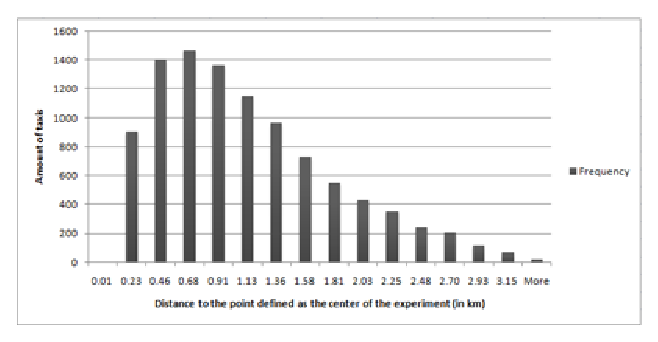
\includegraphics[scale=0.6]{histograma.eps}
	\caption{Histogram with the distribution of taxi drivers in relation to the central point.}
	\label{fig:histograma}
\end{figure}
%
%
\subsection{Service flow}
%
To represent, in a more plausible way the dinamic of real systems, 
it's was built a simulator that represent the changes the position 
of taxi cabs through the city. As the system is built on discrete 
events, these movements occur only after processing a request.

The simulator maintain the approximate reason between the number 
of ocuppied taxis and the amount of vehicles. The test keep on a 
stationary state, with no tendency to increase or decrease
supply in relation to the number of passengers.

A maintanance of taxis in a stationary state guaratee that the 
waiting time keep equal. This analogy derives from the 
relationship proposed by \cite{YANG_WONG}, where the waiting 
time is directly related to amount of spare time of taxi drivers.

Other characteristic of the simulator is related to amendment of
states of taxi drivers. In a real scenario, taxis starts and 
release jobs over the city. To represent this in a discrete way, 
the simulator, after a request processing, modify the availability 
of a few taxi drivers.

It's necessary to inform that elaticity of demand was ignored by 
the simulator. In practice, there is variations of amounts of 
requests due to days of weeks, rush hours, climate conditions, 
among others. However, during the simulation tests, conducted 
under homogeneous conditions, there are no change of the supply of 
services.

As a summary of the procedure used to perform tests, it is possible 
to describe in the following sequence:
%
\begin{enumerate}
	\item The system defines a number N of taxis and puts them 
	random in the city;
	\item Half of the amount of taxis is set as occupied;
	\item Taxi drivers move randomly throughout the city in
	discrete events without changing significantly their
	current position;
	\item Some of the cabs changs your status of "Occupied" to 
	"Free" and vice versa, simulating the being/end of a service;
	\item The algorithm simulates a passenger request;
	\item Each vehicles dispatching system choose the best cab and 
	the time for service is measure for each algorithm;
	\item If the number of request defined for the test is reached 
	yet, the system goes back to the step 3. Else, the system count 
	all the measured times for each algorithm;
\end{enumerate}
%
%
\subsection{Tests conditions}
%
The city of Belo Horizonte (Brazil) was designated as the place 
where the test was realized, simulation a real condition. Due to 
the existence of largest urbanized area in the city center,
with a low number of large green areas and a extensive road network,
the taxi drivers and requests was distributed over the central area 
and vicinity (as the peripherical area).

Besides the actual geographic location where tests were run, 
adjustments were made to the model in order to simulate conditions 
close to the average in the city of Belo Horizonte. The next values 
defines the scenario of the tests: 
%
\begin{itemize}
	\item Average load factor: 50\%;
	\item Maximal numbers of taxis evaluated in circles 
	next to the customer: 7;
	\item "Circle" search radius: 0,7km, 1,2km e 1,5km;
	\item Probability of moving of a taxi: 90\%;
	\item Maximum probability of change the taxi cab status
	("Free" to "Occupied" ou vice versa): 10\%.	
\end{itemize}
%
In the first test, using the real average conditions in Belo 
Horizonte, seted up a representation in witch 300 taxis were 
spread over an area of approximately 34.84 km2. The average 
rate of taxis per km2 was 8.61 or a taxi every 0.12 km2.

In a second test, it was decided to restrict the number of
taxis, in order to analyze the influence of the availability of
services. For that, was defined a amount of 200 taxis in the 
same area (average rate of 5.74 taxis per km2).

%
\subsection{Results}
%

The results of the tests described in this section were
subjected to analysis of variance (One-way ANOVA) followed by 
Tukey test for multiple comparisons averages. We adopted a 
confidence interval of 95\%, with differences being considered 
significant when P<0.05. Statistical analysis was done by 
Graph Pad Prism software (version 5.01).

To reduce the name of the algorithms at the graphics on this 
section, was used the naming standard described at table 
\ref{tab:nomenclatura_algoritmos}.
%
\begin{table}
  \centering
  \begin{tabular}{c|c|c|c|}
    \hline
    %& Tempo de Espera & Dist�ncia Percorrida & Tempo de Processamento \\
    & Time & Distance & Processing \\
    \hline
    %GPS Estimativa Tempo M�nimo & GPS-T & GPS-D & GPS-P \\
    %GPS Dist�ncia Euclidiana & EUC-T & EUC-D & EUC-P \\
    %Broadcasting & BRC-T & BRC-D & BRC-P \\
    (1) & GPS-T & GPS-D & GPS-P \\
    (2) & EUC-T & EUC-D & EUC-P \\
    (3) & BRC-T & BRC-D & BRC-P \\
    \hline
  \end{tabular}
  \caption{Reduced naming pattern of algorithms.}
  \label{tab:nomenclatura_algoritmos}
\end{table}
%
\textbf{\textit{Corrigir tabela (os valores estavam ficando por 
cima da coluna do lado)}}

\textbf{\textit{
\begin{enumerate}
	\item GPS-based algorithm with lower estimated time for service
	\item GPS-based algorithm with Euclidean distance
	\item Broadcasting method
\end{enumerate}
}}

\subsection{Test I}
%
The first result is the customers average time to a taxi service. 
The graph on the figure \ref{fig:tempo_300} show averages times for 
each algorithm.
%
\begin{figure}[!h]
	\centering
	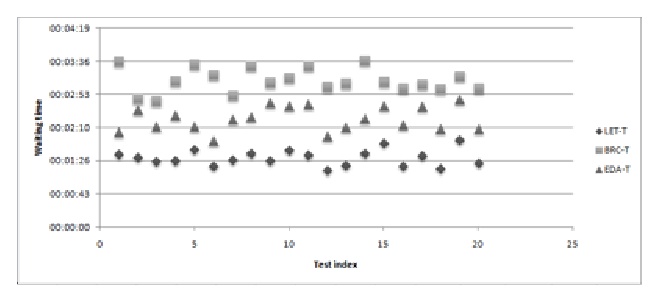
\includegraphics[scale=0.6]{tempo_300.eps}
	\caption{Customer's average time to service.}
	\label{fig:tempo_300}
\end{figure}
%
The GPS-based algorithm with lower estimated time for service had 
lower values, when compared to the GPS-based algorithm with Euclidean 
distance and the Broadcasting method. Therefore it can be inferred, 
according to tests carried out, that this algorithm has lower average 
waiting time to customers. These results were obtained with 95\%
confidence and show that there is a statistically significant, favoring 
the GPS algorithm with Lower Estimate Time for Service.

The results corresponding to the average distance to travel by taxi 
drivers can be seen in figure \ref{fig:distancia_300}.
%
\begin{figure}[!h]
	\centering
	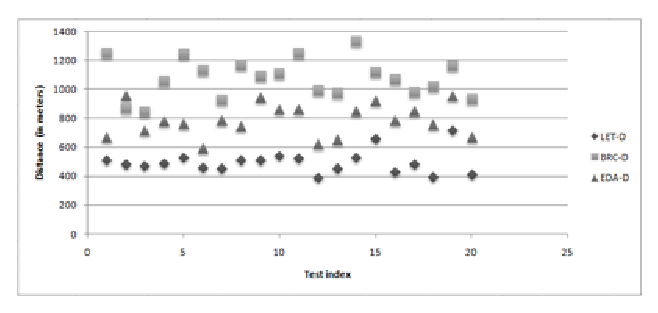
\includegraphics{distancia_300.eps}
	\caption{Taxi average distance to serve a request.}
	\label{fig:distancia_300}
\end{figure}
%
It's possible to see that the average distance traveled by taxi 
drivers in the GPS algorithm is smaller than the distance 
algorithms at EUC and BRC algorithms.

As the proposed tests do not consider traffic information, and 
according to the results, it is possible to correlate the average 
waiting time and the distance traveled by the taxi drivers. As 
already discussed, the average time to serivce is related to 
distance that the driver must go to the customer: the more away 
from the driver, the longer the customer will wait until be 
serviced. The correlation can see in the figure 
\ref{fig:correlacao_300}. 

%
\begin{figure}[h!]
	\centering
	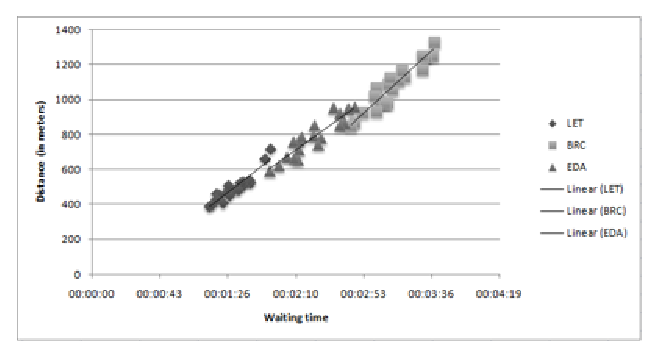
\includegraphics[scale=0.5]{correlacao_300.eps}
	\caption{Correlation between service time and distance.}
	\label{fig:correlacao_300}
\end{figure}
%
Finally, its should evaluate the runtime of the algorithms,
to be able to measure its efficiency in the search for
best taxi available to server the request. The figure 
\ref{fig:execucao_300} show the average time of processing.

%
\begin{figure}[h!]
	\centering
	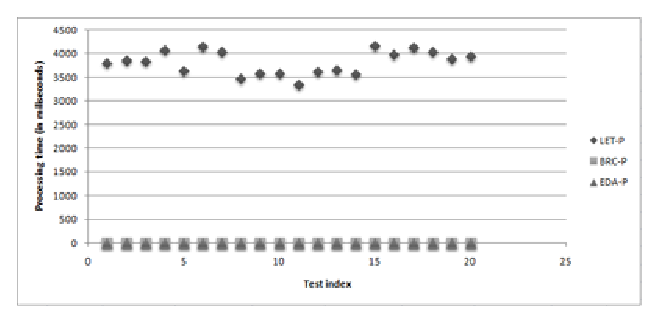
\includegraphics{execucao_300.eps}
	\caption{Average processing time of algorithms.}
	\label{fig:execucao_300}
\end{figure}
%
The analysis of figure \ref{fig:execucao_300} shows that 
the GPS-based algorithm with Euclidean distance and the Broadcasting 
algorithm have significantly lower processing time than GPS-based 
algorithm with lower estimated time for service. 

Despite of the values of processing time of GPS algorithm, when 
compared to the other algorithms, its absolute value is low, 
and it can be used in a real application. Due to the 
characteristics of the algorithm, where the number of processed 
taxi drivers is limited by restrictions of the algorithm and, 
the major time of response is caused by web service calls, it can 
said that the processing time will be stable even with a 
increase of taxis and customers in the a real system.

%
\subsection{Test II: Decrease of taxi avalability}
%
In the second test, we attempted to decrease the supply of 
taxi drivers. To do this, was reduced the number of taxi cabs 
available in the same area of the city. In this second experiment, 
the availability of taxi vehicle was 1 each 0.17 km2.

To evaluate the impact caused by the changes in the test, the 
results of each algorithms, in new conditions, can be seen in 
figure \ref{fig:tempo_200}.
%
\begin{figure}[h!]
	\centering
	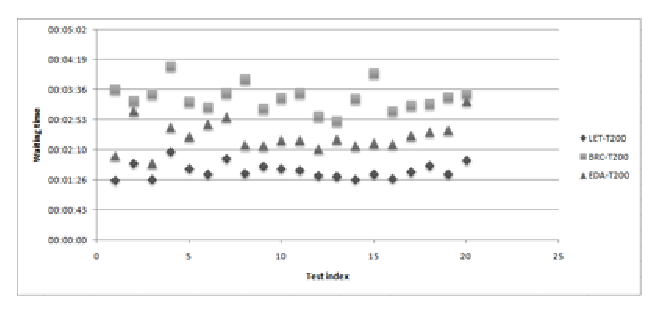
\includegraphics{tempo_200.eps}
	\caption{Customer's average time to service, by each algorithm.}
	\label{fig:tempo_200}
\end{figure}
%
In the second test, at the same as the first one, its possible to 
say, with 95\% that the GPS-based algorithm with lower estimated 
time for service has significantly smaller times than GPS-based 
algorithm with euclidean distance and the broadcasting algorithm.

The results of the average distance to travel by taxi drivers 
in both tests can be seen in figure \ref{fig:distancia_200}
%
\begin{figure}[h!]
	\centering
	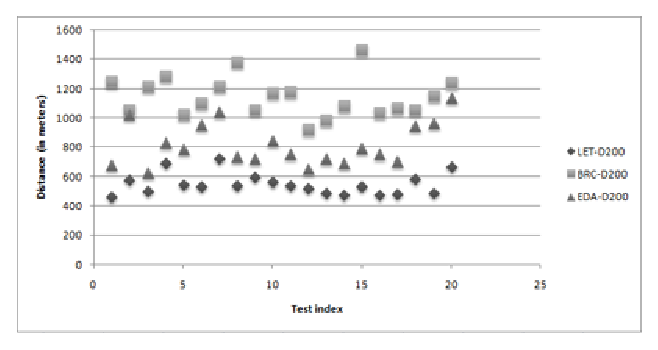
\includegraphics{distancia_200.eps}
	\caption{Taxi average distance to serve a request, by each algorithm.}
	\label{fig:distancia_200}
\end{figure}
%
As in the first test, the average distance traveled by taxi 
drivers in GPS-based algorithm with lower estimated time for 
service is smaller than the distances found in algorithms the 
other algorithms.

%
%
\section{Discussion}
%
The major criterion for the choose of the best algorithm among 
those described in this article is the contribution of each one 
to reduce the average waiting time for taxis services. A second 
criterion used in this article is the computacional cost of each 
algorithm.

In the average waiting time criterion, it's possible to see that 
the GPS-based algorithms had a decrease of at least 25\% when 
compared to the broadcasting algorithm. From a carefull analisys, 
it's possible to know that the GPS-based algorithm with lower 
estimated time for service decrease 52.8\% when compared with 
the broadcasting method. The decrease of time by the GPS-based 
algorithm with euclidean distance is 26.1\%.

In the second test, the software results indicates that the 
reduce of availability of the services decrease the gain of 
the GPS-based algorithms when compared to the broadcasting 
mehtod. The GPS-based algorithm with lower estimated time 
for service was reduced in 51.3\% and the GPS-based 
algorithm with euclidean reduced 27.1\%, when compared to 
the broadcasting algorithm.

As the results in figure \ref{fig:correlacao_300}, it's 
possible to indicate a corelation between the distance to 
travel by the taxi driver and the waiting time for service. 
However, the relation between the both values keeps uniform 
because the traffic conditions was not evaluated in the tests.

In a real scenario, traffic information may cause important 
changes on the values founded. A different route, thats 
is usually slowly, may be the fastest one in a rush hour or 
in bad traffic conditions. But the traffic conditions, may also 
not affect the algorithm. To know the impact of traffic 
conditions on the alogorithms, is necessary to do the 
next analysis:

%
\begin{enumerate}
	\item In a concentrated bad traffic, the speed of congested 
	roads significantly decrease and the linearity of 
	distance-time can be changed: a longer route may be faster 
	than a route that uses congested roads.
	\item In a rush hour, for example, there is a overall 
	decrease of speed of all routes. In this scenario it's 
	not possible to say that rerouting is always justified. 
	In this peek times, it's possible that distance-time 
	corelation keep existing.
\end{enumerate}
%
The response time of the GPS-based algorithm with euclidean 
and the Broadcasting algorithm are similar, with negligible 
value. The response of the GPS-based algorithm with lower 
estimated time for service is significantly slower than other 
algorithms, with average response of 3.8 seconds.

A software it takes to long to respond a request may impact 
the final result of the algorithm, since the cab can move 
through the city. The best vehicle, after a while, can start to 
serve another request or stops to be the best choice, because 
it moves to another direction. A example of how processing 
time can affect the result is a vehicle at 60km/h in a 
1 minute algorithm response: the vehicle may goes 1 km away 
from the point evalueate from the algorithm.

The results of GPS-based algorithms when compared to the 
broadcasting method using computational cost evalution must 
be taken with care, because the broadcasting algorithm don't 
really exists - it's a interaction between taxi drivers and 
the call center operators.

After this alert, it's possible to calculate the impact 
of the slow processig of the GPS-based algorithm with lower 
estimated time for service. In a 60km/h speed, it's impact 
on the original position of the cabs is, at most, 63.3 meters.

%
%
\section{Conclusion}
%
From the study, it's possible to indicate that GPS-based 
algorithms has better results than broadcasting algorithm 
in a waiting time criterion. The results indicate numerically 
that GPS-based methods can improve the quality of services, as 
was expected by \cite{XU_ET_AL}.

Other goal of this work was to indicate the correlation 
between the distance to travel by the cab to serve a request 
and the taxi waiting time. This correlation influences the 
method to choose the best taxi to the client - near taxis 
must decrease the average time of the system.

The analysis of processing time of the algorithms indicates 
that the described algorithms has low response time. Due its 
own characteristics, as well as the times of processing 
found in the simulations, it can be stated that the solutions 
presented have practical feasibility, as the response time 
of the system.

%
%
\section{Future Work}
%
In a future works it's possible to improve the developed 
models, making then closer to the reality. It's is possible 
too consider different environmental conditions in order 
to produce more accurate results. The evaluation of external 
factors to the flow as rain or events, similar to that shown 
by \cite{LIN_ZENG} for predicting bus arrival times can be
used by the algorithm for more accurate results.


% ****************************************************************************
% BIBLIOGRAPHY AREA
% ****************************************************************************



% IF YOU DO NOT USE BIBTEX, USE THE FOLLOWING SAMPLE SCHEME FOR THE REFERENCES
% ----------------------------------------------------------------------------
\begin{thebibliography}{9}

\bibitem{CHENG_QU} S. Cheng and X. Qu, X. A Service Choice Model for Optimizing Taxi Service Delivery,
\emph {Research Collection School of Information Systems}, v. 209, 2009.

\bibitem{LIAO} Z. Liao. Real-Time Taxi Dispatching Using Global Positioning Systems. 
\emph {Communications of ACM}, v. 46, n. 5, may 2009.

\bibitem{XU_ET_AL} Z. Xu, et al. Investigating the Value of Location Information in Taxi Dispatching Services: A case study of DaZhong Taxi. \emph {PACIS 2005 Proceedings}, v. 111, 2005.

\bibitem{RAO_MINAKAKIS} B. Rao and L. Minakakis Evolution of Mobile Location-based Services. \emph{Communications of the ACM - Mobile computing opportunities and challenges}, New York, NY, USA, v. 46 , n. 12, p. 61 - 65, December 2003. ISSN 0001-0782.

\bibitem{YANG_WONG} H. Yang and S. C. Wong. A Network Model of Urban Taxi Services. \emph{Transport Research Board-B}, v. 32, n. 4, p. 235-246, 1998.

\bibitem{LIN_ZENG} W.-H. Lin and J. Zeng. An experimental study on real-time bus arrival - Time prediction with GPS data. \emph{Transportation Research Record}, n. 1666, p. 101-109, 1999. ISSN ISSN: 0361-1981, ISBN 0309070619.

%% For books
%\bibitem{Haykin_book} S. Haykin, editor. \emph{Unsupervised Adaptive Filtering vol. 1: Blind Source Separation}, John Willey ans Sons, New York, 2000.

%% For articles
%\bibitem{DelfosseLoubaton_article}N. Delfosse and P. Loubaton, Adaptibe blind separation of sources: A deflation approach, \emph{Signal Processing}, 45:59--83, Elsevier, 1995.

%% For paper in proceedings published as serie books (LNCS,...)
%\bibitem{CrucCichAmari_bookproceedings} S. Cruces, A. Cichocki and S. Amari, The minimum entropy and cumulants based contrast functions for blind source extraction. In J. Mira and A. Prieto, editors, proceedings of the 6$^{th}$ \emph{international workshop on artificial neural networks} ({IWANN} 2001), Lecture Notes in Computer Science 2085, pages 786-793, Springer-Verlag, 2001.

%% For paper in conference proceedings
%\bibitem{VrinsArchambeau_proceedings} F. Vrins, C. Archambeau and M. Verleysen,Towards a local separation performances estimator using common ICA contrast functions? In M. Verleysen, editor, \emph{proceedings of the $12^{th}$ European Symposium on Artificial Neural Networks} ({ESANN} 2004), d-side pub., pages 211--216, April 28--30, Bruges (Belgium), 2004.

%% For Technical Report
%\bibitem{Stone_TechRep} J. V. Stone and J. Porrill, Under\-complete independent component\vadjust{\eject} analysis for signal separation and dimension reduction. Technical Report, Psychology Department, Sheffield University, Sheffield, S10 2UR, England, October 1997.

\end{thebibliography}
% ----------------------------------------------------------------------------

% IF YOU USE BIBTEX,
% - DELETE THE TEXT BETWEEN THE TWO ABOVE DASHED LINES
% - UNCOMMENT THE NEXT TWO LINES AND REPLACE 'Name_Of_Your_BibFile'

%\bibliographystyle{unsrt}
%\bibliography{Name_Of_Your_BibFile}



% ****************************************************************************
% END OF BIBLIOGRAPHY AREA
% ****************************************************************************

\end{document}

